
\subsection{Kernels estimators}
\paragraph{Some kernels} We list out some common kernels.
\begin{enumerate}
  \item \label{ker:rect} $K\pa{x}=\frac{1}{2}\1_{\abs{x}\le \frac{1}{2}}$ the rectangular
  \item\label{ker:gauss} $K\pa{x} = \frac{1}{\sqrt{2\pi}} e^{-\frac{x^2}{2}}$, the Gaussian kernel
  \item\label{ker:sinc} $K\pa{x} = \frac{\sin\pa{x}}{\pi x}$, the sinc kernel
  \item \label{ker:epan} $K\pa{x} = \frac{3}{4}\max\{0,1-x^2\}=\frac{3}{4}\pa{1-x^2}\1_{\abs{x}\le 1}$, the Epanechnikov kernel
\end{enumerate}
\begin{figure*}[!h]
  \centering
  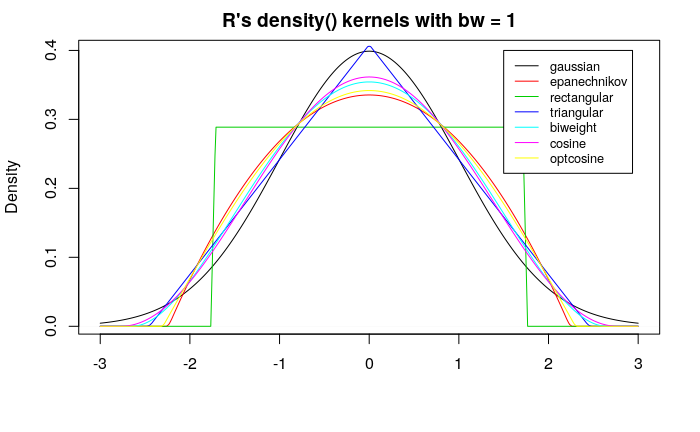
\includegraphics[width=0.8\textwidth]{figures/kernels.png}
  \caption{Kernels}
\end{figure*}
\begin{remark}
  Note that the Gaussian kernel is both in $L^1\pa{\R,\calb\pa{\R},dx}$ and in $L^2\pa{\R,\calb\pa{\R},dx}$. The sinc kernel is only in $L^2\pa{\R,\calb\pa{\R},dx}$ but not in $L^1\pa{\R,\calb\pa{\R},dx}$, as the absolute value fails to be integrable. However, we have
  \begin{equation*}
    1 = \lim_{R\rightarrow \infty}\int_{-R}^R \frac{\sin\pa{x}}{\pi x} dx.
  \end{equation*}
\end{remark}
\begin{remark} The kernel estimator is unbiased when the bandwidth $h$ goes to zero, that is,
  \begin{equation*}
    \begin{split}
      \E\bra{\hat{f}_X\pa{x}} & = \frac{1}{hn}\sum_{i=1}^{n}\E\bra{K\pa{\frac{X_i-x}{h}}}             \\
                              & = \frac{1}{h}\E\bra{K\pa{\frac{X_1-x}{h}}}   \quad \text{by i.i.i.d.} \\
                              & = \frac{1}{h}\int_\R K\pa{\frac{y-x}{h}}f_X\pa{y}dy                   \\
                              & = \frac{1}{h}K\pa{\frac{\cdot}{h}}\ast f_X \pa{x}                     \\
                              & \to f_X(x)
    \end{split}
  \end{equation*}
  It converges in $L^1(\R)$ in the sense that $$\norm{\frac{1}{h}K(\frac{\cdot}{h})\ast f_X-f_X}_1\to 0$$ where $\norm{f}_1=\int_{\R}\abs{f(x)}dx$
\end{remark}
\subsection{Performance analysis}
For a kernel $K$ estimator with bandwidth $h$, we would like to analyze its
performance.
\begin{definition}
  We introduce the quadratic \textbf{risk}
  \begin{equation*}
    \mathrm{MSE}\pa{x} = \E\bra{\pa{\hat{f}_X\pa{x} - f_X\pa{x}}^2},
  \end{equation*}
  where
  \begin{equation*}
    \ell\pa{x,y} = \pa{x-y}^2
  \end{equation*}
  is the \textbf{loss} function.

  Other risks include
  \begin{equation*}
    \E\bra{\sup_{x\in \R} \abs{\hat{f}_X\pa{x}-f_X\pa{x}}} = \E\bra{\norm{\hat{f}_X-f_X }_\infty}
  \end{equation*}
\end{definition}
Note that $\hat{f}_X$ is a function of $x$ and the observations is $X= \pa{X_1,\ldots, X_n}$.

\begin{definition}
  We define the \textbf{bias} of $\hat{f}_X\pa{x}$ by
  \begin{equation*}
    \mathrm{Bias}\pa{\hat{f}_X} = b\pa{x} = \E\bra{\hat{f}_X\pa{x} - f_X\pa{x}}
  \end{equation*}
  and we denote the \textbf{variance} of $\hat{f}_X\pa{x}$ by $\sigma^2\pa{x}$.
\end{definition}

\begin{proposition}
  We have
  \begin{equation*}
    \mathrm{MSE}\pa{x} = b\pa{x}^2 + \sigma^2\pa{x}.
  \end{equation*}
\end{proposition}
\begin{proof}
  We have
  \begin{equation*}
    \begin{split}
      \MSE\pa{x} & = \E\bra{ \pa{\hat{f}_X\pa{x} {\color{red}- \E\bra{\hat{f}_X\pa{x}} + \E\bra{\hat{f}_X\pa{x}}} - f_X\pa{x}}^2}                                                                                              \\
                 & = \E\bra{ \pa{\hat{f}_X\pa{x} - \E\bra{\hat{f}_X\pa{x}}}^2} + 2 \E\bra{\pa{\hat{f}_X\pa{x}- \E\bra{\hat{f}_X\pa{x}}}\underbrace{\pa{\E\bra{\hat{f}_X\pa{x}} - f_X\pa{x}}}_{\text{not random}} }             \\
                 & \quad + \E\bra{\pa{\E\bra{\hat{f}_X\pa{x}} - f_X\pa{x}}^2}                                                                                                                                                  \\
                 & = \underbrace{\E\bra{ \pa{\hat{f}_X\pa{x} - \E\bra{\hat{f}_X\pa{x}}}^2}}_{=\sigma^2\pa{x}} + 2 \pa{\E\bra{\hat{f}_X\pa{x}} - f_X\pa{x}} \underbrace{\E\bra{\hat{f}_X\pa{x}- \E\bra{\hat{f}_X\pa{x}}} }_{=0} \\
                 & \quad + \underbrace{\pa{\E\bra{\hat{f}_X\pa{x}} - f_X\pa{x}}^2}_{=b\pa{x}^2}.                                                                                                                               \\
    \end{split}
  \end{equation*}
\end{proof}

\begin{proposition}[upper bound of $\sigma^2(x)$]\label{prop:1}
  Assume that there exists $f_{\max}\in \R$ such that $\forall x\in \R$, $f_X\pa{x}\leq f_{\max}$ and $\int_\R K^2\pa{u}du <\infty$. Then we have, for any bandwidth $h$, for any $x\in \R$ and for any $n\ge 1$, we have
  \begin{equation*}
    \sigma^2\pa{x}\leq \frac{C}{nh}.
  \end{equation*}
  where $C= f_{\max}\int_\R K^2\pa{u}du$.
\end{proposition}
\begin{proof}
  First observe that, by identical distribution of $X_1,\ldots, X_n$,
  \begin{equation}\label{eq:expectation}
    \E\bra{\hat{f}_X\pa{x}} = \frac{1}{n}\sum_{i=1}^n \frac{1}{h}\E\bra{K\pa{\frac{X_i-x}{h}}} = \frac{1}{h}\E\bra{K\pa{\frac{X_1-x}{h}}}.
  \end{equation}

  Now, using independence in the second line and identical distribution in the
  third line,
  \begin{equation*}
    \begin{split}
      \sigma^2\pa{x} & = \E\bra{\pa{\frac{1}{n} \sum_{i=1}^n \pa{\frac{1}{h} K\pa{\frac{X_i-x}{h}}} - \E\bra{\hat{f}_X \pa{x}}}^2}                   \\
                     & =\E\bra{\frac{1}{n^2}\pa{\sum_{i=1}^n \pa{\frac{1}{h} K\pa{\frac{X_i-x}{h}}}-n\E\bra{\hat{f}_X \pa{x}}}^2}                    \\
                     & =\frac{1}{n^2}\E\bra{\sum_{i=1}^n \pa{\frac{1}{h} K\pa{\frac{X_i-x}{h}}-\E\bra{\hat{f}_X \pa{x}}}^2} \text{ by independence } \\
                     & =\frac{1}{n^2} \sum_{i=1}^n\E\bra{ \pa{\frac{1}{h} K\pa{\frac{X_i-x}{h}} - \E\bra{\hat{f}_X \pa{x}}}^2}                       \\
                     & = \frac{1}{n} \E\bra{\pa{ \frac{1}{h} K\pa{\frac{X_1-x}{h}}- \E\bra{\hat{f}_X \pa{x}}}^2}
    \end{split}
  \end{equation*}
  Inserting equation* \ref{eq:expectation},
  \begin{equation*}
    \begin{split}
      \sigma^2\pa{x} & = \frac{1}{n} \E\bra{\pa{ \frac{1}{h} K\pa{\frac{X_1-x}{h}} - \E\bra{\frac{1}{h} K\pa{\frac{X_1-x}{h}}}}^2}     \\
                     & = \frac{1}{n}\Var\bra{\frac{1}{h} K\pa{\frac{X_1-x}{h}}}                                                        \\
                     & = \frac{1}{n}\pa{ \E\bra{\frac{1}{h^2} K^2\pa{\frac{X_1-x}{h}} } - \E\bra{\frac{1}{h} K\pa{\frac{X_1-x}{h}}}^2} \\
                     & \leq \frac{1}{n} \E\bra{\frac{1}{h^2} K^2\pa{\frac{X_1-x}{h}} }                                                 \\
                     & =\frac{1}{nh} \E\bra{\frac{1}{h} K^2\pa{\frac{X_1-x}{h}} }                                                      \\
                     & =\frac{1}{nh} \int_\R \frac{1}{h} K^2\pa{\frac{y-x}{h}} f_X\pa{y}dy                                             \\
                     & = \frac{1}{nh} \int_\R K^2\pa{u} \underbrace{f_X\pa{x+h u}}_{\leq f_{\max}} du                                  \\
                     & \leq \frac{1}{nh} \underbrace{f_{\max} \int_\R K^2\pa{u} du}_{=C},
    \end{split}
  \end{equation*}
  where we used the change of variables $y=x+hu$.
\end{proof}

\begin{definition}[$\beta$ for a density function]
  Let $\beta>0$, $L>0$ and set $\ell = \lfloor \beta\rfloor$, by which we mean the greatest integer \textbf{strictly} less than $\beta$. The Hölder class $\Sigma \pa{\beta,L}$ is the class of functions $f:\R\rightarrow \R$ such that $f^{\pa{\ell}}$ exists and for all $x,x'\in \R$ we have
  \begin{equation*}
    \abs{f^{\pa{\ell}}\pa{x}- f^{\pa{\ell}}\pa{x'}}\leq L\abs{x-x'}^{\beta -\ell}.
  \end{equation*}
\end{definition}

\begin{definition}
  We define
  \begin{equation*}
    \calp\pa{\beta,L} = \set{f\in\Sigma\pa{\beta,L}: f\geq 0, \int_\R f\pa{x}dx =1}.
  \end{equation*}
\end{definition}
\begin{example}
  $\beta =1$ gives the usual Hölder continuity condition: for all $x,x'\in \R$
  \begin{equation*}
    \abs{f\pa{x}-f\pa{x'}}\leq L\abs{x-x'}^{\beta}.
  \end{equation*}
\end{example}
{\color{blue}
\begin{remark}
  This Hölder condition implies continuity of $f$.
\end{remark}}
\begin{definition}[$\beta$ for a kernel]
  $K:\R\rightarrow \R$ is a kernel \textbf{of order $\ell \in \N_0$} if
  \begin{itemize}
    \item $u\mapsto u^j K\pa{u}$ is integrable for any $j\in\set{0,\ldots,\ell}$,
    \item $\int_\R K\pa{u} du =1$,
    \item and $\int_\R u^j K\pa{u} du =0$ for $j\in\set{1,\ldots, \ell}$.
  \end{itemize}
\end{definition}

\begin{proposition}[upper bound of $\abs{b(x)}$]\label{prop:2}
  Let $f_X\in \calp\pa{\beta,L}$ with $\beta,L >0$ and $K$ of order $\ell \geq \lfloor \beta \rfloor$ such that
  \begin{equation*}
    \int_\R \abs{u}^\beta \abs{K\pa{u}}du <\infty.
  \end{equation*}
  Then, for all $x\in\R$, $n\geq 1$ and $h>0$, we have
  \begin{equation*}
    \abs{b\pa{x}}\leq C_1 h^\beta,
  \end{equation*}
  where
  \begin{equation*}
    C_1 = \frac{L}{\ell !}\int_\R\abs{u}^{\beta} \abs{K\pa{u}} du.
  \end{equation*}
\end{proposition}
\begin{proof}
  Reusing equation \ref{eq:expectation} and using $1= \int_\R K\pa{u}du$ ,
  \begin{equation*}
    \begin{split}
      b\pa{x} & = \E\bra{\hat{f}_X\pa{x}} - f_X\pa{x}                                                \\
              & = \frac{1}{h}\E\bra{K\pa{\frac{X_1-x}{h}}} - f_X\pa{x}                               \\
              & = \frac{1}{h}\int_\R K\pa{\frac{y-x}{h}} f_X\pa{y}dy - f_X\pa{x}                     \\
              & = \frac{1}{h}\int_\R K\pa{\frac{y-x}{h}} f_X\pa{y}dy - \int_\R K\pa{u} f_X\pa{x} du.
    \end{split}
  \end{equation*}
  With the change of variables $y = hu + x$, we obtain
  \begin{equation*}
    \begin{split}
      b\pa{x} & = \int_\R K\pa{u} f_X\pa{hu+x}du - \int_\R K\pa{u} f_X\pa{x} du \\
              & = \int_\R K\pa{u} \pa{f_X\pa{hu +x} - f_X\pa{x}} du.
    \end{split}
  \end{equation*}
  By a Taylor expansion, for some $\tau \in [0,1]$, we obtain
  \begin{equation*}
    f_X\pa{hu+x} - f_X\pa{x} = uh f_X'\pa{x} + \cdots  + \frac{\pa{uh}^{\ell -1}}{\pa{\ell -1}!} f_X^{\pa{\ell -1}}\pa{x}+ \frac{\pa{uh}^\ell}{\ell !}f_X^{\pa{\ell}}\pa{x+\tau uh }.
  \end{equation*}
  Thus, recalling that $\int_\R u^j K\pa{u} du = 0$ for $j\in \set{1,\ldots, \ell}$ (we use it in the second and the third step),
  \begin{equation*}
    \begin{split}
      b\pa{x} & = \int_\R K\pa{u} \pa{uh f_X'\pa{x} + \cdots  + \frac{\pa{uh}^{\ell -1}}{\pa{\ell -1}!} f_X^{\pa{\ell -1}}\pa{x}+ \frac{\pa{uh}^\ell}{\ell !}f_X^{\pa{\ell}}\pa{x+\tau uh }} du \\
              & = \int_\R K\pa{u} \frac{\pa{uh}^\ell}{\ell !}f_X^{\pa{\ell}}\pa{x+\tau uh } du                                                                                                  \\
              & = \int_\R K\pa{u} \frac{\pa{uh}^\ell}{\ell !} \pa{ f_X^{\pa{\ell}}\pa{x+\tau uh } - f_X^{\pa{\ell}}\pa{x}} du.
    \end{split}
  \end{equation*}
  Taking absolute values, using the Hölder property $f_X\in \calp\pa{\beta, L}$, and recalling finally $0\leq \tau \leq 1$,
  \begin{equation*}
    \begin{split}
      \abs{b\pa{x}} & = \abs{\int_\R K\pa{u} \frac{\pa{uh}^\ell}{\ell !} \pa{ f_X^{\pa{\ell}}\pa{x+\tau uh } - f_X^{\pa{\ell}}\pa{x}} du}      \\
                    & \leq \int_\R \abs{K\pa{u}} \frac{\abs{uh}^\ell}{\ell !} \abs{ f_X^{\pa{\ell}}\pa{x+\tau uh } - f_X^{\pa{\ell}}\pa{x}} du \\
                    & \leq \int_\R \abs{K\pa{u}} \frac{\abs{uh}^\ell}{\ell !} L\abs{\tau u h}^{\beta - \ell} du                                \\
                    & = \int_\R \abs{K\pa{u}}  \frac{L\abs{uh}^{\beta}}{\ell !} \abs{\tau}^{\beta - \ell} du                                   \\
                    & \leq  \int_\R \abs{K\pa{u}}  \frac{L\abs{uh}^{\beta}}{\ell !} du                                                         \\
                    & = \frac{L h^\beta}{\ell !}\int_\R \abs{K\pa{u}}\abs{u}^{\beta} du.\end{split}
  \end{equation*}
  This shows the claim.
\end{proof}
\begin{remark}
  Note that the expectation
  \begin{equation*}
    \E\bra{\hat{f}_X\pa{x}} = \frac{1}{h}\int_\R K\pa{\frac{y-x}{h}} f_X\pa{y}dy
  \end{equation*}
  is the \textbf{convolution} $\frac{1}{h} K\pa{\frac{- \pa{\cdot}}{h}}\ast f_X$.

  In general, the convolution of two integrable functions $f,g:\R\rightarrow \R$
  is defined as
  \begin{equation*}
    \pa{f\ast g}\pa{x} = \int_\R f\pa{x-y} g\pa{y} dy.
  \end{equation*}

  One interpretation of the convolution is the following: if $f_X,f_Y$ are the
  densities of independent random variables $X,Y$, then the density of $X+Y$ is
  $f_X\ast f_Y$.

  Indeed, let $\varphi$ be bounded and continuous. Then, using independence and
  writing $u=x+y$, and using Fubini-Tonelli,
  \begin{equation*}
    \begin{split}
      \E\bra{\varphi\pa{X+Y}} & =\int_{\R\times \R} \varphi \pa{x+y} f_{X,Y}\pa{x,y} dx dy  \\
                              & = \int_\R \int_\R \varphi\pa{x+y}f_X\pa{x}f_Y\pa{y} dx dy   \\
                              & = \int_\R \int_\R \varphi\pa{u} f_X\pa{y-u} f_Y\pa{y} du dy \\
                              & = \int_\R \int_\R \varphi\pa{u} f_X\pa{y-u}f_Y\pa{y} dy du  \\
                              & =\int_\R \varphi\pa{u}\int_\R f_X\pa{y-u}f_Y\pa{y} dy du    \\
                              & =\int_\R \varphi\pa{u} f_X\ast f_Y \pa{u} du.
    \end{split}
  \end{equation*}
  This characterises the density uniquely.

  Another way to see this is to consider the characteristic function, which is
  the Fourier transform of the random variable, using independence:
  \begin{equation*}
    \E\bra{e^{it\pa{X+Y}}} = \E\bra{e^{itX}e^{itY}} = \E\bra{e^{itX}}\E\bra{e^{itY}}.
  \end{equation*}
  The latter is the product of the characteristic functions of $X$ and $Y$. The very same expression as on the right-hand side is yielded taking the characteristic function of a random variable with density $f_X\ast f_Y$, and the characteristic function characterises the distribution uniquely.
\end{remark}
\paragraph{Result}
Combining proposition \ref{prop:1} and \ref{prop:2}, we see
\begin{equation*}
  \MSE \pa{x}\leq C_1^2 h^{2\beta} + \frac{C}{nh}.
\end{equation*}
Minimizing the right-hand side in $h$ yields $h_{\opt}= \pa{\frac{C}{2\beta C_1^2 n}}^{\frac{1}{2\beta +1}}\sim n^{-\frac{1}{2\beta +1}}$.

Plugging this back into the right-hand side, we obtain
\begin{equation*}
  \MSE\pa{x} = O\pa{n^{-\frac{2\beta}{2\beta+1}}}.
\end{equation*}
